\documentclass[border=5pt]{standalone}

% ---- Fonts (match main paper) ----
\usepackage[T1]{fontenc}
\usepackage{newtxtext}
\usepackage[amssymbols]{newtxmath}

% ---- Packages ----
\usepackage{amsmath}
\usepackage{tikz}
\usetikzlibrary{arrows.meta,calc,decorations.markings}
\usepackage{pgfplots}
\pgfplotsset{compat=1.18}
\usepackage{booktabs}
\usepackage{tcolorbox}
\tcbuselibrary{skins}

\begin{document}

\begin{tcolorbox}[
  title={\bfseries Example: An Optimal $(n{=}3,\; M{=}4)$ Code for
         Bernoulli$(0.3)$},
  width=16cm,
  colback=white,
  colframe=black!70,
  coltitle=white,
  fonttitle=\bfseries\sffamily,
  arc=2mm,
  boxrule=0.8pt,
  top=6pt,
  bottom=6pt,
  left=5pt,
  right=5pt,
]

% =====================================================================
%  TOP ROW: PANELS (a) AND (b) SIDE BY SIDE
% =====================================================================
\begin{minipage}[t]{0.46\linewidth}
\centering
\textbf{\textsf{(a)}\; Encoding on the Hamming Cube $\{0,1\}^3$}\par\vspace{8pt}
%
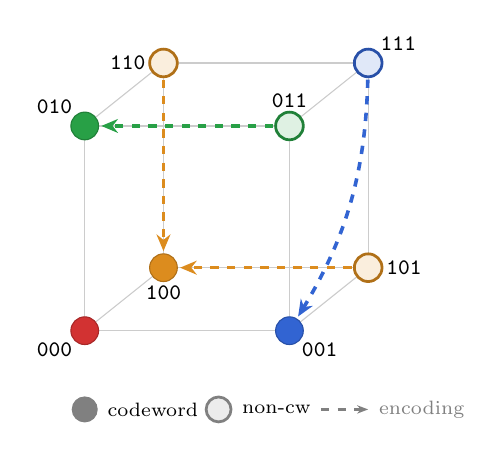
\begin{tikzpicture}[
  scale=1,
  % --- node styles ---
  cw/.style={circle, draw=#1!80!black, fill=#1,
             minimum size=10pt, inner sep=0pt},
  ncw/.style={circle, draw=#1!80!black, fill=#1!15,
              minimum size=10pt, inner sep=0pt, line width=1pt},
  enc/.style={-{Stealth[length=6pt,width=5pt]},
              dashed, #1, line width=1.3pt,
              shorten >=6pt, shorten <=6pt},
  lbl/.style={font=\footnotesize\ttfamily},
]
  % --- Codeword colours ---
  \definecolor{cRed}{RGB}{210,50,50}
  \definecolor{cBlue}{RGB}{50,100,210}
  \definecolor{cGreen}{RGB}{40,160,70}
  \definecolor{cOrange}{RGB}{220,140,30}

  % --- Cube vertex coordinates ---
  % bit1 (leftmost) = depth, bit2 = vertical, bit3 = horizontal
  \def\sx{2.6}   % horizontal span (bit 3)
  \def\sy{2.6}   % vertical   span (bit 2)
  \def\ddx{1.0}  % depth x-offset  (bit 1)
  \def\ddy{0.8}  % depth y-offset  (bit 1)

  % Back face (bit 1 = 0)
  \coordinate (v000) at (0, 0);
  \coordinate (v001) at (\sx, 0);
  \coordinate (v010) at (0, \sy);
  \coordinate (v011) at (\sx, \sy);
  % Front face (bit 1 = 1)
  \coordinate (v100) at (\ddx, \ddy);
  \coordinate (v101) at ({\sx+\ddx}, \ddy);
  \coordinate (v110) at (\ddx, {\sy+\ddy});
  \coordinate (v111) at ({\sx+\ddx}, {\sy+\ddy});

  % --- Cube edges (thin gray) ---
  % Back face
  \draw[gray!40, thin] (v000) -- (v001);
  \draw[gray!40, thin] (v001) -- (v011);
  \draw[gray!40, thin] (v011) -- (v010);
  \draw[gray!40, thin] (v010) -- (v000);
  % Front face
  \draw[gray!40, thin] (v100) -- (v101);
  \draw[gray!40, thin] (v101) -- (v111);
  \draw[gray!40, thin] (v111) -- (v110);
  \draw[gray!40, thin] (v110) -- (v100);
  % Depth edges
  \draw[gray!40, thin] (v000) -- (v100);
  \draw[gray!40, thin] (v001) -- (v101);
  \draw[gray!40, thin] (v010) -- (v110);
  \draw[gray!40, thin] (v011) -- (v111);

  % --- Codeword nodes (filled) ---
  \node[cw=cRed]    at (v000) {};
  \node[cw=cBlue]   at (v001) {};
  \node[cw=cGreen]  at (v010) {};
  \node[cw=cOrange] at (v100) {};

  % --- Non-codeword nodes (lightly filled, coloured by assigned codeword) ---
  \node[ncw=cGreen]  at (v011) {};   % -> 010
  \node[ncw=cOrange] at (v101) {};   % -> 100
  \node[ncw=cOrange] at (v110) {};   % -> 100
  \node[ncw=cBlue]   at (v111) {};   % -> 001

  % --- Encoding arrows (drawn LAST so they appear on top) ---
  % 011 -> 010  (green, d_H = 1)
  \draw[enc=cGreen]  (v011) -- (v010);
  % 101 -> 100  (orange, d_H = 1)
  \draw[enc=cOrange] (v101) -- (v100);
  % 110 -> 100  (orange, d_H = 1)
  \draw[enc=cOrange] (v110) -- (v100);
  % 111 -> 001  (blue, d_H = 2)
  \draw[enc=cBlue]   (v111) to[bend left=15] (v001);

  % --- Vertex labels ---
  \node[lbl, below left=1pt]  at (v000) {000};
  \node[lbl, below right=1pt] at (v001) {001};
  \node[lbl, above left=1pt]  at (v010) {010};
  \node[lbl, above=3pt]       at (v011) {011};
  \node[lbl, below=3pt]       at (v100) {100};
  \node[lbl, right=3pt]       at (v101) {101};
  \node[lbl, left=3pt]        at (v110) {110};
  \node[lbl, above right=1pt] at (v111) {111};

  % --- Legend ---
  \node[circle, draw=gray, fill=gray, minimum size=9pt, inner sep=0pt,
        label={[font=\scriptsize]right:codeword}]
    at (0, -1.0) {};
  \node[circle, draw=gray, fill=gray!15, minimum size=9pt, inner sep=0pt,
        line width=1pt,
        label={[font=\scriptsize]right:non-cw}]
    at (1.7, -1.0) {};
  \draw[dashed, gray, line width=1.2pt, -{Stealth[length=4pt,width=3pt]}]
    (3.0, -1.0) -- (3.6, -1.0)
    node[right, font=\scriptsize] {encoding};
\end{tikzpicture}
\end{minipage}%
\hfill
% =====================================================================
%  PANEL (b): ENCODING TABLE
% =====================================================================
\begin{minipage}[t]{0.51\linewidth}
\centering
\textbf{\textsf{(b)}\; Encoding Table}\par\vspace{8pt}
%
\small
\renewcommand{\arraystretch}{1.15}
\begin{tabular}{@{}ccccc@{}}
\toprule
Source $x^3$ & $p(x^3)$ & Codeword $\hat{c}$ & Output & $d/n$ \\
\midrule
\texttt{000} & $0.343$ & \texttt{000} & \texttt{00} & $0$ \\
\texttt{001} & $0.147$ & \texttt{001} & \texttt{01} & $0$ \\
\texttt{010} & $0.147$ & \texttt{010} & \texttt{10} & $0$ \\
\texttt{100} & $0.147$ & \texttt{100} & \texttt{11} & $0$ \\
\addlinespace[3pt]
\texttt{011} & $0.063$ & \texttt{010} & \texttt{10} & $1/3$ \\
\texttt{101} & $0.063$ & \texttt{100} & \texttt{11} & $1/3$ \\
\texttt{110} & $0.063$ & \texttt{100} & \texttt{11} & $1/3$ \\
\texttt{111} & $0.027$ & \texttt{001} & \texttt{01} & $2/3$ \\
\bottomrule
\end{tabular}

\vspace{8pt}
{\footnotesize
The encoder transmits $\log_2 4 = 2$ bits per block of $n = 3$ source symbols.}

\vspace{8pt}
\begin{gather*}
R = \tfrac{1}{n}\log_2 M
  = \tfrac{2}{3}
  \approx 0.667 \;\text{bit/sym} \\[4pt]
\bar{D}
  = \sum_{x^3} p(x^3)\,\frac{d(x^3,\,\hat{c})}{n}
  = 0.081
\end{gather*}
\end{minipage}

\vspace{8pt}
\noindent\rule{\linewidth}{0.4pt}
\vspace{6pt}

% =====================================================================
%  PANEL (c): MINI R(D) CURVE
% =====================================================================
\centering
\textbf{\textsf{(c)}\; Comparison with the Shannon Limit}\par\vspace{4pt}
%
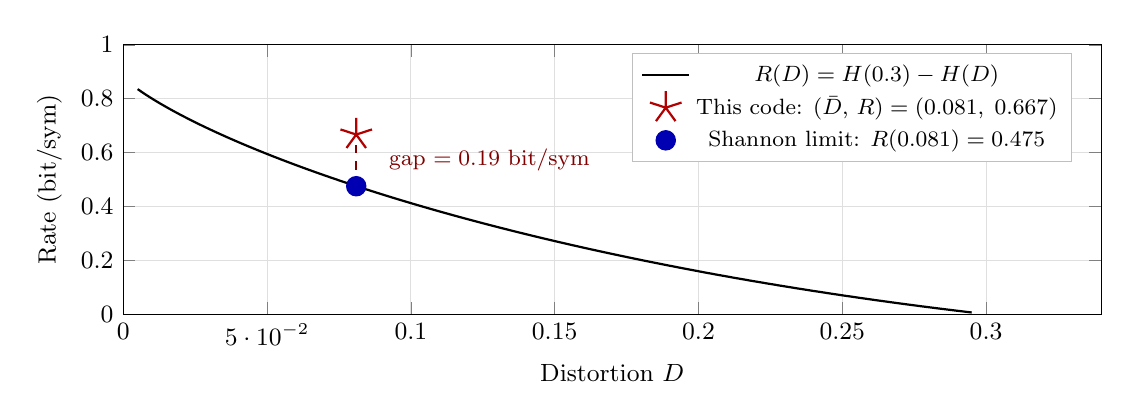
\begin{tikzpicture}
\begin{axis}[
  width=14cm,
  height=5cm,
  xlabel={Distortion $D$},
  ylabel={Rate (bit/sym)},
  xmin=0, xmax=0.34,
  ymin=0, ymax=1.0,
  grid=major,
  grid style={gray!25, thin},
  legend pos=north east,
  legend style={font=\footnotesize, draw=gray!50},
  tick label style={font=\small},
  label style={font=\small},
  xtick={0, 0.05, 0.10, 0.15, 0.20, 0.25, 0.30},
]

% --- R(D) = H(0.3) - H(D) curve ---
\addplot[
  domain=0.005:0.295,
  samples=200,
  thick,
  black,
] {0.8813 + x*ln(x)/ln(2) + (1-x)*ln(1-x)/ln(2)};
\addlegendentry{$R(D) = H(0.3) - H(D)$}

% --- Our code: star marker ---
\addplot[
  only marks,
  mark=star,
  mark size=6pt,
  mark options={fill=red!70!black, draw=red!70!black, thick},
] coordinates {(0.081, 0.667)};
\addlegendentry{This code: $(\bar{D},\,R) = (0.081,\; 0.667)$}

% --- Shannon limit: filled circle ---
\addplot[
  only marks,
  mark=*,
  mark size=3.5pt,
  mark options={fill=blue!70!black, draw=blue!70!black},
] coordinates {(0.081, 0.475)};
\addlegendentry{Shannon limit: $R(0.081) = 0.475$}

% --- Gap annotation ---
\draw[dashed, thick, red!50!black]
  (axis cs:0.081, 0.475) -- (axis cs:0.081, 0.667);
\node[font=\footnotesize, right, text=red!50!black]
  at (axis cs:0.089, 0.571) {gap $= 0.19$ bit/sym};

\end{axis}
\end{tikzpicture}

\vspace{4pt}
{\small This finite code operates $0.19$ bit/sym above the Shannon limit ---
Section~6 quantifies how this gap shrinks as the block length $n$ grows.}

\end{tcolorbox}

\end{document}
